%% Creator: Inkscape inkscape 0.48.1, www.inkscape.org
%% PDF/EPS/PS + LaTeX output extension by Johan Engelen, 2010
%% Accompanies image file 'df.ps' (pdf, eps, ps)
%%
%% To include the image in your LaTeX document, write
%%   \input{<filename>.pdf_tex}
%%  instead of
%%   \includegraphics{<filename>.pdf}
%% To scale the image, write
%%   \def\svgwidth{<desired width>}
%%   \input{<filename>.pdf_tex}
%%  instead of
%%   \includegraphics[width=<desired width>]{<filename>.pdf}
%%
%% Images with a different path to the parent latex file can
%% be accessed with the `import' package (which may need to be
%% installed) using
%%   \usepackage{import}
%% in the preamble, and then including the image with
%%   \import{<path to file>}{<filename>.pdf_tex}
%% Alternatively, one can specify
%%   \graphicspath{{<path to file>/}}
%% 
%% For more information, please see info/svg-inkscape on CTAN:
%%   http://tug.ctan.org/tex-archive/info/svg-inkscape

\begingroup
  \makeatletter
  \providecommand\color[2][]{%
    \errmessage{(Inkscape) Color is used for the text in Inkscape, but the package 'color.sty' is not loaded}
    \renewcommand\color[2][]{}%
  }
  \providecommand\transparent[1]{%
    \errmessage{(Inkscape) Transparency is used (non-zero) for the text in Inkscape, but the package 'transparent.sty' is not loaded}
    \renewcommand\transparent[1]{}%
  }
  \providecommand\rotatebox[2]{#2}
  \ifx\svgwidth\undefined
    \setlength{\unitlength}{506.22191162pt}
  \else
    \setlength{\unitlength}{\svgwidth}
  \fi
  \global\let\svgwidth\undefined
  \makeatother
  \begin{picture}(1,0.85806523)%
    \put(0,0){\includegraphics[width=\unitlength]{df.ps}}%
    \put(0.037,0.13358698){\color[rgb]{0,0,0}\makebox(0,0)[lb]{\smash{0}}}%
    \put(0.037,0.822){\color[rgb]{0,0,0}\makebox(0,0)[lb]{\smash{1}}}%
    \put(0.02011223,0.50050621){\color[rgb]{0,0,0}\rotatebox{90}{\makebox(0,0)[lb]{\smash{$f$}}}}%
    \put(0.05662929,0.0824032){\color[rgb]{0,0,0}\makebox(0,0)[lb]{\smash{$10^{-3}$}}}% 
    \put(0.22866002,0.08239394){\color[rgb]{0,0,0}\makebox(0,0)[lb]{\smash{$10^{-2}$}}}%

   
    \put(0.40610898,0.08239394){\color[rgb]{0,0,0}\makebox(0,0)[lb]{\smash{$10^{-1}$}}}%
    \put(0.58829901,0.08239394){\color[rgb]{0,0,0}\makebox(0,0)[lb]{\smash{$10^{0}$}}}%
    \put(0.76507068,0.08239394){\color[rgb]{0,0,0}\makebox(0,0)[lb]{\smash{$10^1$}}}%
    \put(0.93868178,0.08239394){\color[rgb]{0,0,0}\makebox(0,0)[lb]{\smash{$10^2$}}}%
    \put(0.48,-0){\color[rgb]{0,0,0}\makebox(0,0)[lb]{\smash{$T$\,(эВ)}}}%
    \put(0.75,0.76939719){\color[rgb]{0,0,0}\makebox(0,0)[lb]{\smash{$t=0$\,с}}}%
    \put(0.75,0.71107162){\color[rgb]{0,0,0}\makebox(0,0)[lb]{\smash{$t=1$\,мкс}}}%
  \end{picture}%
\endgroup
